\documentclass[12pt]{article}
\usepackage{natbib}
\usepackage{eso-pic}
\usepackage{amsmath} % flere matematikkommandoer
\usepackage{amssymb}
\usepackage[utf8]{inputenc} % æøå
\usepackage[T1]{fontenc} % mere æøå
\usepackage[danish]{babel} % orddeling
\usepackage{verbatim} % så man kan skrive ren tekst
\usepackage[a4paper, margin = 1in]{geometry}
\usepackage{graphicx}
\usepackage{placeins}
\author{
  Christian Kjær Larsen\\
  \texttt{011292} \\[.4cm]
  Lukas Svarre Engedal\\
  \texttt{210790} \\[.4cm]
  Tobias Sønderskov Hansen\\
  \texttt{whg656@alumni.ku.dk} \\[.4cm]
  Instruktor: Aske Mottelson\\[.4cm]
  \vspace{10cm}
}

\title{
  \vspace{3cm}
  \Huge{ProjDat 2015} \\[.25cm]
  \large{Delrapport 1}
}

\begin{document}

\AddToShipoutPicture*{\put(0,0){\includegraphics*[viewport=0 0 700 600]{includes/nat-farve}}}
\AddToShipoutPicture*{\put(0,602){\includegraphics*[viewport=0 600 700 1600]{includes/nat-farve}}}

%% Change `ku-en` to `nat-en` to use the `Faculty of Science` header
\AddToShipoutPicture*{\put(0,0){\includegraphics*{includes/nat-en}}}

\clearpage\maketitle
\thispagestyle{empty}

\newpage

\tableofcontents %generate table of content

\thispagestyle{empty}

\newpage
\pagestyle{plain}
\setcounter{page}{1}
\pagenumbering{arabic}

\section{Problemformulering}
Opbygningen af problemformuleringen er beskrevet på figur 14-11 i \cite{OOSE}. Vi har i vores beskrivelse de samme punkter.
\subsection{Problemområde}
Fra næste år af laver de markant om på datalogi uddannelsen, og i den forbindelse slår de bl.a. kurserne \emph{Introduktion til Programmering} og \emph{Objektorienteret programmering og design} sammen til et nyt kursus, hvor de i stedet for SML og Java vil bruge F\#.
I den forbindelse forudser kursuslederne at det muligvis kan blive svært at finde tilstrækkeligt med instruktorer til at hjælpe de studerende med at lære og løse opgaver i F\#, og kursuslederne vil derfor gerne have automatiseret hele opgaveaspektet så vidt muligt.

I den forbindelse har de bedt os om at hjælpe dem med at lave et slags interaktivt læringssystem, hvor de studerende kan logge ind og løse en række opgaver der skal hjælpe dem med at lære F\#, og hvor de kan få hints til opgaverne hvis de har brug for det. Opgaverne er grupperede efter emner og sværhedsgrad sådan at de studerende kan starte med de simpleste og de nemmeste opgaver og så efterhånden som de klarer sig igennem dem og bliver bedre kan de gå videre til de mere avancerede og svære opgaver.

Derudover skal kursuslederne gerne nemt kunne tilføje nye og ændre eller fjerne eksisterende spørgsmål, og de skal derudover gerne have adgang til en form for statistik over hvordan de studerende klarer de forskellige opgaver sådan at de kan se hvor der måske er mangler, enten i selve opgaverne eller måske mere alvorligt i undervisningen.

Hvis der bliver tid og overskud til det kan hele opgave aspektet også forbedres ved såkaldt gamification, sådan at de studerende motiveres til at lave flere opgaver på forskellige måneder. Det kunne f.eks. være ved at belønne dem for at løse opgaver ved at give dem point for hver opgave de gennemfører, lade dem optjene badges for at gennemføre hele grupper af opgaver samt give dem mulighed for at sammenligne deres egne præstationer med deres venners og medstuderendes for at skabe et aspekt af konkurrence.


\subsection{Scenarier}
I problemformuleringen skal indgå en række overordnede scenarier, som beskriver den generelle brug af systemet. Dette er med udgangspunkt i afsnit 4.4.2 i \cite{OOSE}. De er lidt mere generelle end dem i bogen, men dette er for at holde designet af systemet åbent for senere ændringer.
\paragraph{Tilføjelse af spørgsmål}
En underviser på kurset går ind på hjemmesiden. Vedkommende logger ind på siden, og han tages til en speciel side for administatorer.
Her skal han tilføje en ny opgave. Vedkommende giver spørgsmålet en kategori efter hvilket læringsmål det opfylder. Opgavesteksten og de rigtige svar skrives ind. Eventuelt tilføjes hints.

\paragraph{Løsning af opgaver}
En studerende på kurset logger ind på hjemmesiden, vedkommende tages til en side, hvor man ser alle læringsmålene, og hvad man allerede har opfyldt. Den studerende vælger et af de tilgængelige læringsmål, og en side åbnes hvor man kan besvare en ny opgave inden for emnet. Den studerende svarer på spørgsmålet, og får feedback med det samme, og der er mulighed for hints, hvis spørgsmålet er svært.

\paragraph{Tjek af log}
En underviser på kurset logger ind på hjemmesiden. Vedkommende vil gerne se, om de studerende har svært ved nogle af emnerne. Der findes et menupunkt der hedder \emph{Log}. Her ses en oversigt over spørgsmålene, og hvilke spørgsmål der bliver svaret ofte forkert på.

\subsection{Funktionelle krav}
De funktionelle krav for systemet er i tråd med afsnit 4.3.1 i \cite{OOSE}, nemlig at de omhandler den specifikke brug af systemet.
\begin{itemize}
    \item Systemet skal være en hjemmeside med opgaver, som kan løses individuelt af studerende.
    \item Der kræves login, så man kan følge med i den studerendes udvikling.
    \item Sprøgsmålene skal være grupperede efter hvilke læringsmål de tester.
    \item Læringsmålene skal igen grupperes efter et \emph{threshold}, som er et øvre læringsmål hvorefter der kommer sværere stof.
    \item Der skal være hints til opgaverne, og der skal kunne gives feedback til hintsne.
    \item Alle forsøg på opgavebesvarelser skal gemmes i en log.
\end{itemize}
Hvis der er tid i en af de senere iterationer, så er der en række ekstra krav som kan implementeres.
\begin{itemize}
    \item Loggen skal bruges til at give underviseren information om hvilke spørgsmål der er svære.
    \item Der skal tilføjes en grad af \emph{gamification}, så der gives badges og point for fremskridt, og det bliver muligt at følge med i andres fremskridt.
    \item Hvis man ikke har øvet sig i et emne i et stykke tid, så falder ens erfaring i området.
\end{itemize}
\subsection{Ikke-funktionelle krav}
De ikke-funktionelle krav til dette projekt er forholdsvis begrænsede. Vi har ret stor frihed i forhold til vores kunde. I afsnit 4.3.2 i \cite{OOSE} beskrives ikke-funktionelle krav som krav, der ikke direkte beskriver funktionaliteten, men mere generelle krav omkring ting som brugervenlighed, ydeevne, pålidelighed og hvor vedligeholdesesvenligt systemet er.

I vores tilfælde er det vigtigste krav er at det skal være nemt at tilføje nye opgaver til systemet, sådan at kursuslederne efterfølgende kan opbygge en tilstrækkelig samling af opgaver til de studerende.

Derudover er det også et mere overordnet krav at det endelige produkt gerne skal være så simpelt og modulært som muligt, sådan at det er nemt at overtage, udvide og bygge videre på efter at vi overgiver projektet til kunden. Ingen af kunderne er web-udviklere, så det er også vigtigt at det valgte framework er veldokumenteret og rimeligt simpelt at bruge.
\subsection{Implementeringsmiljø}
\begin{itemize}
\item Studenter skal kunne bruge læringssystemet ved hjælp af en webbrowser der understøtter JavaScript.
\item Det endelige system skal kunne køre på KU's servere.
\end{itemize}

\section{Indledende projektplan}
Opbygningen af projektplanen er baseret på afsnittene i \cite{OOSE} af samme navn, specifikt punktet på side 568 og figur 14-9. Da der er tale om en indledende projektplan og mange af tingene ikke er helt lagt fast endnu har vi lavet en kort skitse af flere af punkterne.
\subsection{Projektoversigt}
Projektet omhandler udvikling af en webapplikation. Den skal understøtte undervisningen på førsteårskurset i programmering på DIKU. Applikationen skal hjælpe studerende med at forstå kernestof, ved at stille opgaver tilhørende de forskellige læringsmål. Underviserne skal så kunne tilføje nye opgaver, og indhente statistik på allerede stillede opgaver.
\subsection{Resultatbeskrivelse}
Til sidst i projektet er målet, at vi afleverer et fungerende system til kunden. Til prototypen skal der også være en mængde dokumentation til kunden, så vedkommende ved, hvordan løsningen er sammensat.
Til kurset skal vi aflevere en mængde delrapporter, som dokumenterer vores arbejde i løbet af projektet.
\subsection{Arbejdsfordeling}
På nuværende tidspunkt er det svært at sige en masse om arbejdsfordelingen, umiddelbart er vi alle tre interesserede i opgaven og dens forskellige aspekter og vil gerne deltage i dem alle, men hen af vejen finder vi måske ud af at opdele opgaven imellem os ud fra interesser og kompetencer.
\subsection{Køreplan}
Vores køreplan er at følge den plan der er fastlagt i kurset i forhold til hvornår vi skal have prototyper og rapporter klar, og derudover vil vi forsøge så vidt muligt at arbejde i iterationer af f.eks. 2 ugers varighed hvor vi tilføjer funktionalitet modulvis.
\subsection{Risikohåndtering}
Under udviklingsprocessen holder vi jævnligt møder, hvor vi snakker om hvor langt vi er nået. Dette kan bruges til at opdage, om noget af det er udvikles kan udgøre et problem i fremtiden. Det kan være, at to moduler, som to personer udvikler hver for sig, måske ikke er helt kompatible. Det kan også være at man har undervurderet tiden en opgave tager, og der så skal bruges mere tid, eller flere udviklere.


\section{System og softwarearkitektur}
Da det endelige system er en webapplikation, så giver det nogle forudbestemte delsystemer, som traditionelt knytter sig til webudvikling.
\subsection{Delsystemer}
\begin{itemize}
    \item Der skal være et delsystem, som tager sig af opbevaring af vedvarende data. Det er fx opgaver, brugere og en log over besvarelser. Det vil nok være en databaseserver.
    \item Der skal også være et delsystem, der tager sig af forretningslogikken. Der er i vores tilfælde nok en webserver, som tager imod forespørgsler fra brugere, og kommunikerer med databasen. Den vil nok også stå for at lave HTML, der vises i brugerens webbrowser. Det er forskelligt alt efter hvilken platform man vælger, hvordan det skal struktureres.
    \item Brugerens webbrowser er også et undersystem. Det sørger for at sende forespørgsler til vores webserver, og præsentere den returnerede HTML. Det er også her at designprocessen foregår, altså den store treenighed, nemlig HTML, CSS og JavaScript.
\end{itemize}
Det er også det, der traditionelt giver en klar rollefordeling i webudvikling, hvor man har frontend, som består i designet af brugerfladen i HTML, CSS og JavaScript. Der er backend, som igen består af databaseudvikling og udvikling af services og logik som frontenden så bruger.

\section{Projektaftalen}
\subsection{Kontakt}
I dette projekt er vi så heldige at vores kunder, Martin Dybdal og Oleksandr Shturmov, har kontorer lige ovre i B-bygningen på H. C. Ørstedsinstituttet, og det er derfor meget nemt og hurtigt at mødes når vi aftaler det. Derfor tænker vi også frem for at have en fast aftale om at mødes f.eks. én gang om måneden eller hver anden uge at vi bare aftaler at mødes løbende når vi har noget at mødes om. Det kunne f.eks. være hvis vi har spørgsmål til kunden eller omvendt, eller hvis vi har færdiggjort et stykke kode eller en feature som vi gerne vil vise frem og have respons på. Samtidig vil vi selfølgelig også stile efter at der ikke går mere end to uger mellem at vi mødes sådan at vi alle er med på og enige i hvad der foregår og skal foregå.

\subsection{Slutprodukt}
Det endelige produkt vi har aftalt at vi skal aflevere med vores kunde er et læringssystem der er så færdiggjort og rigt på features som muligt. Til at starte med stiler vi naturligvis imod at producere et fungerende system hvor alle de grundlæggende elementer er på plads, altså et system hvor de studerende kan logge ind og løse opgaver i F\# og hvor de kursusansvarlige kan administrere systemet. Derudover er der så yderligere en lang række forslag til ekstra features som vi vil forsøge at implementere så mange af som muligt for at udvide og berige systemet, men som ikke direkte er krav. Planen er så at kunden kan overtage systemet fra os og selv arbejde videre på det og videreudvikle det.


\section{Intern projektetablering}
\subsection{Kommunikationsformer}
Vi bruger email til kommunikation, både internt i gruppen, og med klienten. På den måde er det nemt at overskue al kommunikation, der er foregået omkring projektet.
Derudover tilstræber vi internt i gruppen, at mødes ca. en gang ugentligt, hvor vi snakker om projektet og får overblik over rapportskrivningen.
\subsection{Arbejdssstyring}
Internt i gruppen bruger vi Git til versionsstyring af alle dokumenter og kildekode. Så er det nemt at holde styr på hvad der er lavet, og vi kan arbejde på projektet uafhængigt af hinanden. Vi arbejder også agilt, da det er et krav i forbindelse med projektet. Det betyder at vi under projektet ender med en serie af prototyper, hver med mere funktionalitet end den forrige.

\section{Afleveringsopgaver}
\subsection{OOSE 1.6}
\begin{itemize}
\item "The TicketDistributor must enable a traveler to buy weekly passes.",	funktionelt krav, da det beskriver en konkret opgave systemet skal kunne løse.
\item "The TicketDistributor must be written in Java.", dette er et krav til selve platformen systemet skal køre på, hvilket altså er et ikke-funktionelt krav.
\item "The TicketDistributor must be easy to use.", krav til systemets brugervenlighed, dvs. et ikke-funktionelt krav.
\item "The TicketDistributor must always be available.", dette er et ikke-funktionelt krav, da det har med systemets tilgængelighed at gøre.
\item "The TicketDistributor must provide a phone number to call when it fails.", ikke-funktionelt krav, da det beskriver hvordan systemet skal håndtere fejl.
\end{itemize}
\subsection{OOSE 1.8}
Første gang account nævnes er det som et application domain koncept. Sætningen beskriver at et system skal håndtere nogle kunders bankkontoer, her er accounts altså ikke en del af selve systemet. Efterfølgende bruges account som et solution domain koncept. Teksten er her en diskussion af systemets design, hvor account refererer til systemets repræsentation af en brugers bankkonto.
\subsection{OOSE 2.(6, 7, 9, 10)}
\subsubsection*{Opgave 2.6}
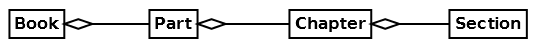
\includegraphics[scale=0.8]{diagrammer/E2_6} \\
\subsubsection*{Opgave 2.7}
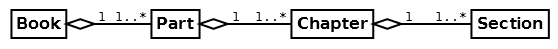
\includegraphics[scale=0.8]{diagrammer/E2_7} \\
\subsubsection*{Opgave 2.9}
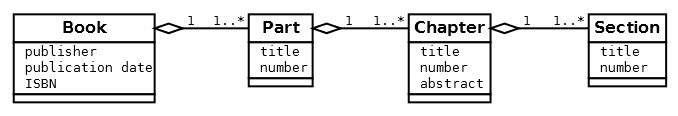
\includegraphics[scale=0.8]{diagrammer/E2_9} \\
\subsubsection*{Opgave 2.10}
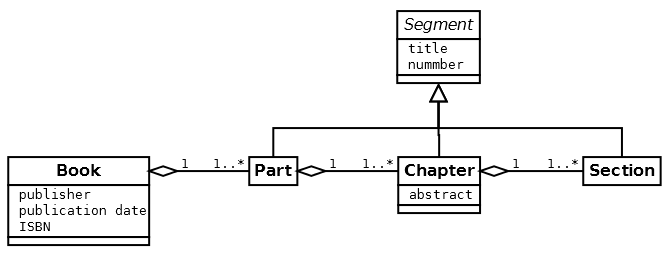
\includegraphics[scale=0.8]{diagrammer/E2_10} \\
\subsection{OOSE 5.3}
Sekvensdiagram med to controllere er vist herunder. Den ene håndterer input fra brugeren, og den anden håndterer input på et lavere niveau. Det kan være fra window manageren, men det kan også være fra netværk eller andet. \\
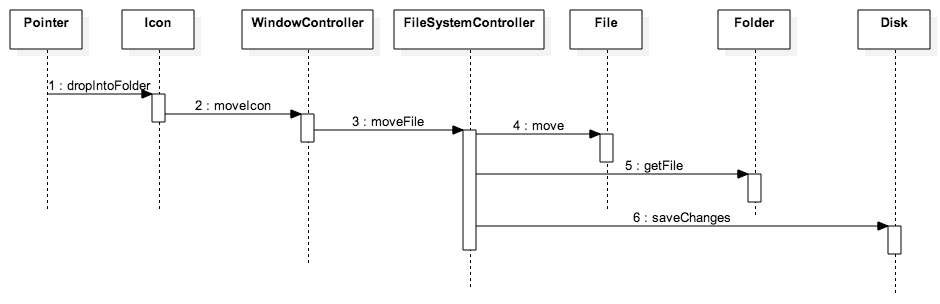
\includegraphics[width=1.0\textwidth]{diagrammer/SD.png}
\subsection{OOSE 7.1}
Deploymentdiagram til opgave 7.1 \\
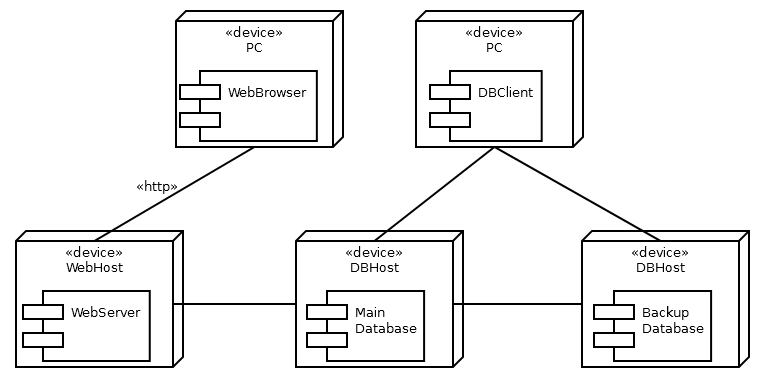
\includegraphics[scale=0.8]{diagrammer/E7_1} \\
\bibliographystyle{alpha}
\bibliography{refs}{}
\end{document}
